% Created by tikzDevice version 0.12.3.1 on 2023-04-19 11:05:19
% !TEX encoding = UTF-8 Unicode
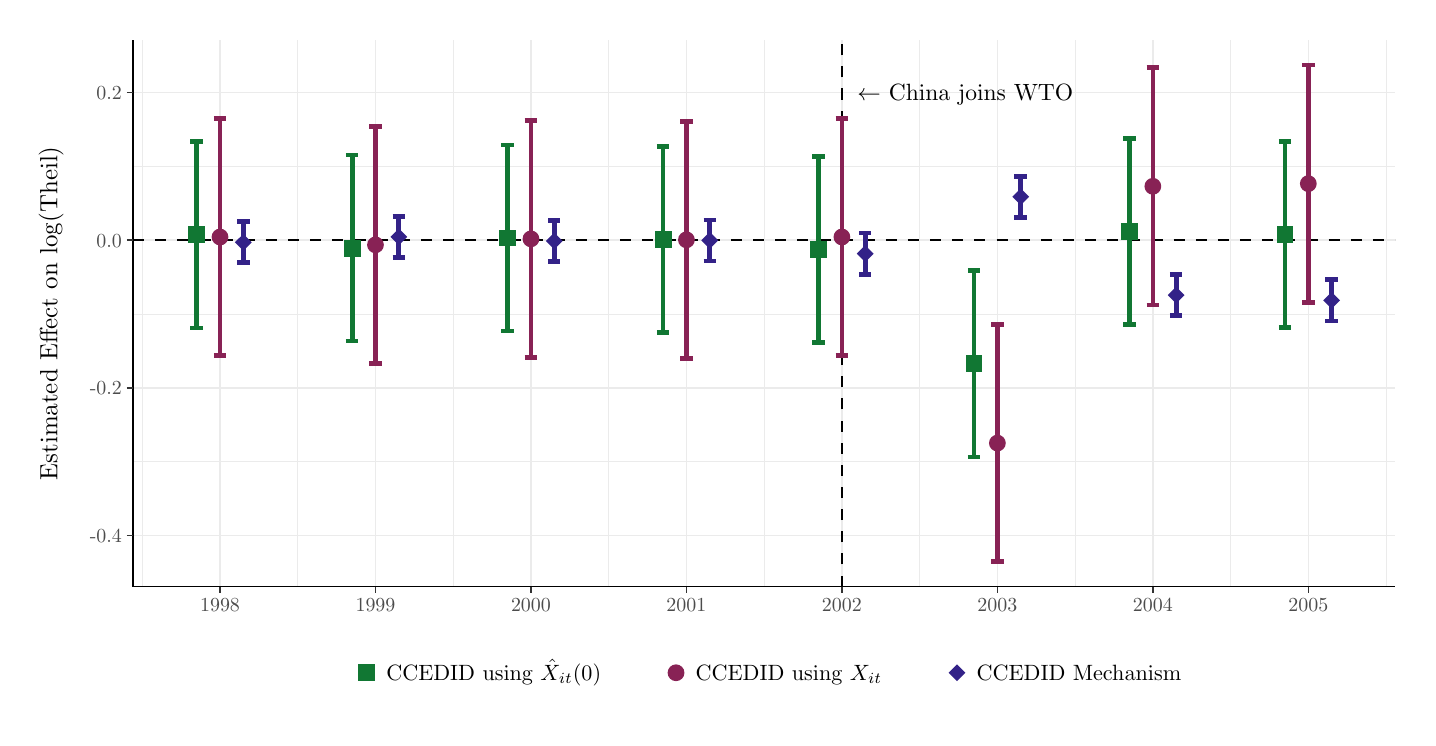
\begin{tikzpicture}[x=1pt,y=1pt]
\definecolor{fillColor}{RGB}{255,255,255}
\path[use as bounding box,fill=fillColor] (0,0) rectangle (498.66,249.33);
\begin{scope}
\path[clip] (  0.00,  0.00) rectangle (498.66,249.33);
\definecolor{drawColor}{RGB}{255,255,255}

\path[draw=drawColor,line width= 0.5pt,line join=round,line cap=round,fill=fillColor] ( -0.00,  0.00) rectangle (498.66,249.33);
\end{scope}
\begin{scope}
\path[clip] ( 38.10, 47.36) rectangle (494.16,244.83);
\definecolor{fillColor}{RGB}{255,255,255}

\path[fill=fillColor] ( 38.10, 47.36) rectangle (494.16,244.83);
\definecolor{drawColor}{gray}{0.92}

\path[draw=drawColor,line width= 0.2pt,line join=round] ( 38.10, 92.50) --
	(494.16, 92.50);

\path[draw=drawColor,line width= 0.2pt,line join=round] ( 38.10,145.87) --
	(494.16,145.87);

\path[draw=drawColor,line width= 0.2pt,line join=round] ( 38.10,199.23) --
	(494.16,199.23);

\path[draw=drawColor,line width= 0.2pt,line join=round] ( 41.41, 47.36) --
	( 41.41,244.83);

\path[draw=drawColor,line width= 0.2pt,line join=round] ( 97.59, 47.36) --
	( 97.59,244.83);

\path[draw=drawColor,line width= 0.2pt,line join=round] (153.77, 47.36) --
	(153.77,244.83);

\path[draw=drawColor,line width= 0.2pt,line join=round] (209.95, 47.36) --
	(209.95,244.83);

\path[draw=drawColor,line width= 0.2pt,line join=round] (266.13, 47.36) --
	(266.13,244.83);

\path[draw=drawColor,line width= 0.2pt,line join=round] (322.31, 47.36) --
	(322.31,244.83);

\path[draw=drawColor,line width= 0.2pt,line join=round] (378.49, 47.36) --
	(378.49,244.83);

\path[draw=drawColor,line width= 0.2pt,line join=round] (434.67, 47.36) --
	(434.67,244.83);

\path[draw=drawColor,line width= 0.2pt,line join=round] (490.85, 47.36) --
	(490.85,244.83);

\path[draw=drawColor,line width= 0.5pt,line join=round] ( 38.10, 65.81) --
	(494.16, 65.81);

\path[draw=drawColor,line width= 0.5pt,line join=round] ( 38.10,119.18) --
	(494.16,119.18);

\path[draw=drawColor,line width= 0.5pt,line join=round] ( 38.10,172.55) --
	(494.16,172.55);

\path[draw=drawColor,line width= 0.5pt,line join=round] ( 38.10,225.92) --
	(494.16,225.92);

\path[draw=drawColor,line width= 0.5pt,line join=round] ( 69.50, 47.36) --
	( 69.50,244.83);

\path[draw=drawColor,line width= 0.5pt,line join=round] (125.68, 47.36) --
	(125.68,244.83);

\path[draw=drawColor,line width= 0.5pt,line join=round] (181.86, 47.36) --
	(181.86,244.83);

\path[draw=drawColor,line width= 0.5pt,line join=round] (238.04, 47.36) --
	(238.04,244.83);

\path[draw=drawColor,line width= 0.5pt,line join=round] (294.22, 47.36) --
	(294.22,244.83);

\path[draw=drawColor,line width= 0.5pt,line join=round] (350.40, 47.36) --
	(350.40,244.83);

\path[draw=drawColor,line width= 0.5pt,line join=round] (406.58, 47.36) --
	(406.58,244.83);

\path[draw=drawColor,line width= 0.5pt,line join=round] (462.76, 47.36) --
	(462.76,244.83);
\definecolor{drawColor}{RGB}{0,0,0}

\path[draw=drawColor,line width= 0.6pt,dash pattern=on 4pt off 4pt ,line join=round] ( 38.10,172.55) -- (494.16,172.55);

\path[draw=drawColor,line width= 0.6pt,dash pattern=on 4pt off 4pt ,line join=round] (294.22, 47.36) -- (294.22,244.83);

\node[text=drawColor,anchor=base west,inner sep=0pt, outer sep=0pt, scale=  0.85] at (299.84,222.98) {$\leftarrow$ China joins WTO};
\definecolor{drawColor}{RGB}{17,119,51}

\path[draw=drawColor,line width= 1.7pt,line join=round] ( 58.83,208.07) --
	( 63.32,208.07);

\path[draw=drawColor,line width= 1.7pt,line join=round] ( 61.07,208.07) --
	( 61.07,140.85);

\path[draw=drawColor,line width= 1.7pt,line join=round] ( 58.83,140.85) --
	( 63.32,140.85);

\path[draw=drawColor,line width= 1.7pt,line join=round] (115.01,203.29) --
	(119.50,203.29);

\path[draw=drawColor,line width= 1.7pt,line join=round] (117.25,203.29) --
	(117.25,136.06);

\path[draw=drawColor,line width= 1.7pt,line join=round] (115.01,136.06) --
	(119.50,136.06);

\path[draw=drawColor,line width= 1.7pt,line join=round] (171.19,206.93) --
	(175.68,206.93);

\path[draw=drawColor,line width= 1.7pt,line join=round] (173.43,206.93) --
	(173.43,139.71);

\path[draw=drawColor,line width= 1.7pt,line join=round] (171.19,139.71) --
	(175.68,139.71);

\path[draw=drawColor,line width= 1.7pt,line join=round] (227.37,206.36) --
	(231.86,206.36);

\path[draw=drawColor,line width= 1.7pt,line join=round] (229.61,206.36) --
	(229.61,139.14);

\path[draw=drawColor,line width= 1.7pt,line join=round] (227.37,139.14) --
	(231.86,139.14);

\path[draw=drawColor,line width= 1.7pt,line join=round] (283.54,202.81) --
	(288.04,202.81);

\path[draw=drawColor,line width= 1.7pt,line join=round] (285.79,202.81) --
	(285.79,135.59);

\path[draw=drawColor,line width= 1.7pt,line join=round] (283.54,135.59) --
	(288.04,135.59);

\path[draw=drawColor,line width= 1.7pt,line join=round] (339.72,161.46) --
	(344.22,161.46);

\path[draw=drawColor,line width= 1.7pt,line join=round] (341.97,161.46) --
	(341.97, 94.24);

\path[draw=drawColor,line width= 1.7pt,line join=round] (339.72, 94.24) --
	(344.22, 94.24);

\path[draw=drawColor,line width= 1.7pt,line join=round] (395.90,209.18) --
	(400.40,209.18);

\path[draw=drawColor,line width= 1.7pt,line join=round] (398.15,209.18) --
	(398.15,141.96);

\path[draw=drawColor,line width= 1.7pt,line join=round] (395.90,141.96) --
	(400.40,141.96);

\path[draw=drawColor,line width= 1.7pt,line join=round] (452.08,208.32) --
	(456.58,208.32);

\path[draw=drawColor,line width= 1.7pt,line join=round] (454.33,208.32) --
	(454.33,141.10);

\path[draw=drawColor,line width= 1.7pt,line join=round] (452.08,141.10) --
	(456.58,141.10);
\definecolor{drawColor}{RGB}{136,34,85}

\path[draw=drawColor,line width= 1.7pt,line join=round] ( 67.25,216.57) --
	( 71.75,216.57);

\path[draw=drawColor,line width= 1.7pt,line join=round] ( 69.50,216.57) --
	( 69.50,130.80);

\path[draw=drawColor,line width= 1.7pt,line join=round] ( 67.25,130.80) --
	( 71.75,130.80);

\path[draw=drawColor,line width= 1.7pt,line join=round] (123.43,213.73) --
	(127.93,213.73);

\path[draw=drawColor,line width= 1.7pt,line join=round] (125.68,213.73) --
	(125.68,127.96);

\path[draw=drawColor,line width= 1.7pt,line join=round] (123.43,127.96) --
	(127.93,127.96);

\path[draw=drawColor,line width= 1.7pt,line join=round] (179.61,215.89) --
	(184.11,215.89);

\path[draw=drawColor,line width= 1.7pt,line join=round] (181.86,215.89) --
	(181.86,130.12);

\path[draw=drawColor,line width= 1.7pt,line join=round] (179.61,130.12) --
	(184.11,130.12);

\path[draw=drawColor,line width= 1.7pt,line join=round] (235.79,215.55) --
	(240.29,215.55);

\path[draw=drawColor,line width= 1.7pt,line join=round] (238.04,215.55) --
	(238.04,129.79);

\path[draw=drawColor,line width= 1.7pt,line join=round] (235.79,129.79) --
	(240.29,129.79);

\path[draw=drawColor,line width= 1.7pt,line join=round] (291.97,216.58) --
	(296.47,216.58);

\path[draw=drawColor,line width= 1.7pt,line join=round] (294.22,216.58) --
	(294.22,130.81);

\path[draw=drawColor,line width= 1.7pt,line join=round] (291.97,130.81) --
	(296.47,130.81);

\path[draw=drawColor,line width= 1.7pt,line join=round] (348.15,142.10) --
	(352.65,142.10);

\path[draw=drawColor,line width= 1.7pt,line join=round] (350.40,142.10) --
	(350.40, 56.34);

\path[draw=drawColor,line width= 1.7pt,line join=round] (348.15, 56.34) --
	(352.65, 56.34);

\path[draw=drawColor,line width= 1.7pt,line join=round] (404.33,234.89) --
	(408.83,234.89);

\path[draw=drawColor,line width= 1.7pt,line join=round] (406.58,234.89) --
	(406.58,149.12);

\path[draw=drawColor,line width= 1.7pt,line join=round] (404.33,149.12) --
	(408.83,149.12);

\path[draw=drawColor,line width= 1.7pt,line join=round] (460.51,235.86) --
	(465.01,235.86);

\path[draw=drawColor,line width= 1.7pt,line join=round] (462.76,235.86) --
	(462.76,150.09);

\path[draw=drawColor,line width= 1.7pt,line join=round] (460.51,150.09) --
	(465.01,150.09);
\definecolor{drawColor}{RGB}{51,34,136}

\path[draw=drawColor,line width= 1.7pt,line join=round] ( 75.68,179.18) --
	( 80.17,179.18);

\path[draw=drawColor,line width= 1.7pt,line join=round] ( 77.93,179.18) --
	( 77.93,164.35);

\path[draw=drawColor,line width= 1.7pt,line join=round] ( 75.68,164.35) --
	( 80.17,164.35);

\path[draw=drawColor,line width= 1.7pt,line join=round] (131.86,181.15) --
	(136.35,181.15);

\path[draw=drawColor,line width= 1.7pt,line join=round] (134.11,181.15) --
	(134.11,166.31);

\path[draw=drawColor,line width= 1.7pt,line join=round] (131.86,166.31) --
	(136.35,166.31);

\path[draw=drawColor,line width= 1.7pt,line join=round] (188.04,179.65) --
	(192.53,179.65);

\path[draw=drawColor,line width= 1.7pt,line join=round] (190.29,179.65) --
	(190.29,164.82);

\path[draw=drawColor,line width= 1.7pt,line join=round] (188.04,164.82) --
	(192.53,164.82);

\path[draw=drawColor,line width= 1.7pt,line join=round] (244.22,179.88) --
	(248.71,179.88);

\path[draw=drawColor,line width= 1.7pt,line join=round] (246.47,179.88) --
	(246.47,165.05);

\path[draw=drawColor,line width= 1.7pt,line join=round] (244.22,165.05) --
	(248.71,165.05);

\path[draw=drawColor,line width= 1.7pt,line join=round] (300.40,175.09) --
	(304.89,175.09);

\path[draw=drawColor,line width= 1.7pt,line join=round] (302.65,175.09) --
	(302.65,160.26);

\path[draw=drawColor,line width= 1.7pt,line join=round] (300.40,160.26) --
	(304.89,160.26);

\path[draw=drawColor,line width= 1.7pt,line join=round] (356.58,195.65) --
	(361.07,195.65);

\path[draw=drawColor,line width= 1.7pt,line join=round] (358.83,195.65) --
	(358.83,180.82);

\path[draw=drawColor,line width= 1.7pt,line join=round] (356.58,180.82) --
	(361.07,180.82);

\path[draw=drawColor,line width= 1.7pt,line join=round] (412.76,160.12) --
	(417.25,160.12);

\path[draw=drawColor,line width= 1.7pt,line join=round] (415.01,160.12) --
	(415.01,145.29);

\path[draw=drawColor,line width= 1.7pt,line join=round] (412.76,145.29) --
	(417.25,145.29);

\path[draw=drawColor,line width= 1.7pt,line join=round] (468.94,158.21) --
	(473.43,158.21);

\path[draw=drawColor,line width= 1.7pt,line join=round] (471.19,158.21) --
	(471.19,143.38);

\path[draw=drawColor,line width= 1.7pt,line join=round] (468.94,143.38) --
	(473.43,143.38);
\definecolor{fillColor}{RGB}{17,119,51}

\path[fill=fillColor] ( 58.04,171.43) --
	( 64.11,171.43) --
	( 64.11,177.49) --
	( 58.04,177.49) --
	cycle;

\path[fill=fillColor] (114.22,166.64) --
	(120.29,166.64) --
	(120.29,172.71) --
	(114.22,172.71) --
	cycle;

\path[fill=fillColor] (170.40,170.29) --
	(176.47,170.29) --
	(176.47,176.35) --
	(170.40,176.35) --
	cycle;

\path[fill=fillColor] (226.58,169.72) --
	(232.65,169.72) --
	(232.65,175.79) --
	(226.58,175.79) --
	cycle;

\path[fill=fillColor] (282.76,166.17) --
	(288.83,166.17) --
	(288.83,172.24) --
	(282.76,172.24) --
	cycle;

\path[fill=fillColor] (338.94,124.82) --
	(345.00,124.82) --
	(345.00,130.88) --
	(338.94,130.88) --
	cycle;

\path[fill=fillColor] (395.12,172.54) --
	(401.18,172.54) --
	(401.18,178.60) --
	(395.12,178.60) --
	cycle;

\path[fill=fillColor] (451.30,171.68) --
	(457.36,171.68) --
	(457.36,177.74) --
	(451.30,177.74) --
	cycle;
\definecolor{fillColor}{RGB}{136,34,85}

\path[fill=fillColor] ( 69.50,173.68) circle (  3.03);

\path[fill=fillColor] (125.68,170.85) circle (  3.03);

\path[fill=fillColor] (181.86,173.01) circle (  3.03);

\path[fill=fillColor] (238.04,172.67) circle (  3.03);

\path[fill=fillColor] (294.22,173.69) circle (  3.03);

\path[fill=fillColor] (350.40, 99.22) circle (  3.03);

\path[fill=fillColor] (406.58,192.01) circle (  3.03);

\path[fill=fillColor] (462.76,192.97) circle (  3.03);
\definecolor{fillColor}{RGB}{51,34,136}

\path[fill=fillColor] ( 74.89,171.77) --
	( 77.93,174.80) --
	( 80.96,171.77) --
	( 77.93,168.73) --
	cycle;

\path[fill=fillColor] (131.07,173.73) --
	(134.11,176.76) --
	(137.14,173.73) --
	(134.11,170.70) --
	cycle;

\path[fill=fillColor] (187.25,172.23) --
	(190.29,175.27) --
	(193.32,172.23) --
	(190.29,169.20) --
	cycle;

\path[fill=fillColor] (243.43,172.47) --
	(246.47,175.50) --
	(249.50,172.47) --
	(246.47,169.43) --
	cycle;

\path[fill=fillColor] (299.61,167.67) --
	(302.65,170.71) --
	(305.68,167.67) --
	(302.65,164.64) --
	cycle;

\path[fill=fillColor] (355.79,188.23) --
	(358.83,191.27) --
	(361.86,188.23) --
	(358.83,185.20) --
	cycle;

\path[fill=fillColor] (411.97,152.70) --
	(415.01,155.73) --
	(418.04,152.70) --
	(415.01,149.67) --
	cycle;

\path[fill=fillColor] (468.15,150.80) --
	(471.19,153.83) --
	(474.22,150.80) --
	(471.19,147.76) --
	cycle;
\end{scope}
\begin{scope}
\path[clip] (  0.00,  0.00) rectangle (498.66,249.33);
\definecolor{drawColor}{RGB}{0,0,0}

\path[draw=drawColor,line width= 0.5pt,line join=round] ( 38.10, 47.36) --
	( 38.10,244.83);
\end{scope}
\begin{scope}
\path[clip] (  0.00,  0.00) rectangle (498.66,249.33);
\definecolor{drawColor}{gray}{0.30}

\node[text=drawColor,anchor=base east,inner sep=0pt, outer sep=0pt, scale=  0.72] at ( 34.05, 63.33) {-0.4};

\node[text=drawColor,anchor=base east,inner sep=0pt, outer sep=0pt, scale=  0.72] at ( 34.05,116.70) {-0.2};

\node[text=drawColor,anchor=base east,inner sep=0pt, outer sep=0pt, scale=  0.72] at ( 34.05,170.07) {0.0};

\node[text=drawColor,anchor=base east,inner sep=0pt, outer sep=0pt, scale=  0.72] at ( 34.05,223.44) {0.2};
\end{scope}
\begin{scope}
\path[clip] (  0.00,  0.00) rectangle (498.66,249.33);
\definecolor{drawColor}{gray}{0.20}

\path[draw=drawColor,line width= 0.5pt,line join=round] ( 35.85, 65.81) --
	( 38.10, 65.81);

\path[draw=drawColor,line width= 0.5pt,line join=round] ( 35.85,119.18) --
	( 38.10,119.18);

\path[draw=drawColor,line width= 0.5pt,line join=round] ( 35.85,172.55) --
	( 38.10,172.55);

\path[draw=drawColor,line width= 0.5pt,line join=round] ( 35.85,225.92) --
	( 38.10,225.92);
\end{scope}
\begin{scope}
\path[clip] (  0.00,  0.00) rectangle (498.66,249.33);
\definecolor{drawColor}{RGB}{0,0,0}

\path[draw=drawColor,line width= 0.5pt,line join=round] ( 38.10, 47.36) --
	(494.16, 47.36);
\end{scope}
\begin{scope}
\path[clip] (  0.00,  0.00) rectangle (498.66,249.33);
\definecolor{drawColor}{gray}{0.20}

\path[draw=drawColor,line width= 0.5pt,line join=round] ( 69.50, 45.11) --
	( 69.50, 47.36);

\path[draw=drawColor,line width= 0.5pt,line join=round] (125.68, 45.11) --
	(125.68, 47.36);

\path[draw=drawColor,line width= 0.5pt,line join=round] (181.86, 45.11) --
	(181.86, 47.36);

\path[draw=drawColor,line width= 0.5pt,line join=round] (238.04, 45.11) --
	(238.04, 47.36);

\path[draw=drawColor,line width= 0.5pt,line join=round] (294.22, 45.11) --
	(294.22, 47.36);

\path[draw=drawColor,line width= 0.5pt,line join=round] (350.40, 45.11) --
	(350.40, 47.36);

\path[draw=drawColor,line width= 0.5pt,line join=round] (406.58, 45.11) --
	(406.58, 47.36);

\path[draw=drawColor,line width= 0.5pt,line join=round] (462.76, 45.11) --
	(462.76, 47.36);
\end{scope}
\begin{scope}
\path[clip] (  0.00,  0.00) rectangle (498.66,249.33);
\definecolor{drawColor}{gray}{0.30}

\node[text=drawColor,anchor=base,inner sep=0pt, outer sep=0pt, scale=  0.72] at ( 69.50, 38.35) {1998};

\node[text=drawColor,anchor=base,inner sep=0pt, outer sep=0pt, scale=  0.72] at (125.68, 38.35) {1999};

\node[text=drawColor,anchor=base,inner sep=0pt, outer sep=0pt, scale=  0.72] at (181.86, 38.35) {2000};

\node[text=drawColor,anchor=base,inner sep=0pt, outer sep=0pt, scale=  0.72] at (238.04, 38.35) {2001};

\node[text=drawColor,anchor=base,inner sep=0pt, outer sep=0pt, scale=  0.72] at (294.22, 38.35) {2002};

\node[text=drawColor,anchor=base,inner sep=0pt, outer sep=0pt, scale=  0.72] at (350.40, 38.35) {2003};

\node[text=drawColor,anchor=base,inner sep=0pt, outer sep=0pt, scale=  0.72] at (406.58, 38.35) {2004};

\node[text=drawColor,anchor=base,inner sep=0pt, outer sep=0pt, scale=  0.72] at (462.76, 38.35) {2005};
\end{scope}
\begin{scope}
\path[clip] (  0.00,  0.00) rectangle (498.66,249.33);
\definecolor{drawColor}{RGB}{0,0,0}

\node[text=drawColor,rotate= 90.00,anchor=base,inner sep=0pt, outer sep=0pt, scale=  0.90] at ( 10.70,146.10) {Estimated Effect on $\log($Theil$)$};
\end{scope}
\begin{scope}
\path[clip] (  0.00,  0.00) rectangle (498.66,249.33);
\definecolor{fillColor}{RGB}{255,255,255}

\path[fill=fillColor] (100.94,  4.50) rectangle (431.32, 27.95);
\end{scope}
\begin{scope}
\path[clip] (  0.00,  0.00) rectangle (498.66,249.33);
\definecolor{fillColor}{RGB}{255,255,255}

\path[fill=fillColor] (108.28,  9.00) rectangle (136.74, 23.45);
\end{scope}
\begin{scope}
\path[clip] (  0.00,  0.00) rectangle (498.66,249.33);
\definecolor{fillColor}{RGB}{17,119,51}

\path[fill=fillColor] (119.48, 13.19) --
	(125.54, 13.19) --
	(125.54, 19.26) --
	(119.48, 19.26) --
	cycle;
\end{scope}
\begin{scope}
\path[clip] (  0.00,  0.00) rectangle (498.66,249.33);
\definecolor{fillColor}{RGB}{255,255,255}

\path[fill=fillColor] (220.06,  9.00) rectangle (248.51, 23.45);
\end{scope}
\begin{scope}
\path[clip] (  0.00,  0.00) rectangle (498.66,249.33);
\definecolor{fillColor}{RGB}{136,34,85}

\path[fill=fillColor] (234.28, 16.23) circle (  3.03);
\end{scope}
\begin{scope}
\path[clip] (  0.00,  0.00) rectangle (498.66,249.33);
\definecolor{fillColor}{RGB}{255,255,255}

\path[fill=fillColor] (321.61,  9.00) rectangle (350.06, 23.45);
\end{scope}
\begin{scope}
\path[clip] (  0.00,  0.00) rectangle (498.66,249.33);
\definecolor{fillColor}{RGB}{51,34,136}

\path[fill=fillColor] (332.80, 16.23) --
	(335.83, 19.26) --
	(338.86, 16.23) --
	(335.83, 13.19) --
	cycle;
\end{scope}
\begin{scope}
\path[clip] (  0.00,  0.00) rectangle (498.66,249.33);
\definecolor{drawColor}{RGB}{0,0,0}

\node[text=drawColor,anchor=base west,inner sep=0pt, outer sep=0pt, scale=  0.80] at (129.58, 13.47) {CCEDID using $\hat{X}_{it}(0)$};
\end{scope}
\begin{scope}
\path[clip] (  0.00,  0.00) rectangle (498.66,249.33);
\definecolor{drawColor}{RGB}{0,0,0}

\node[text=drawColor,anchor=base west,inner sep=0pt, outer sep=0pt, scale=  0.80] at (241.35, 13.47) {CCEDID using $X_{it}$};
\end{scope}
\begin{scope}
\path[clip] (  0.00,  0.00) rectangle (498.66,249.33);
\definecolor{drawColor}{RGB}{0,0,0}

\node[text=drawColor,anchor=base west,inner sep=0pt, outer sep=0pt, scale=  0.80] at (342.90, 13.47) {CCEDID Mechanism};
\end{scope}
\end{tikzpicture}
